\section{Normalization of \ac{t2w}-\ac{mri} images} \label{sec:chp5:T2-norm}
This section presents the state-of-the-art method poroposed for normalization of \ac{t2w}-\ac{mri} prostate images.
Our proposed methods (Sect.~\ref{subsec:chp5:T2-norm:meth}), the designed experiments and finally the conclusions drawn from the results obtained. 
 
Artan \textit{et al.}~\cite{Artan2010,Artan2009} and Ozer \textit{et al.}~\cite{Ozer2009,Ozer2010} proposed to normalize the T2W-\ac{mri} images by computing the standard score (i.e., \textit{z-score}) of the \ac{pz} pixels such as: 
\begin{equation}
  I_{s}(x) = \frac{I_{r}(x) - \mu_{PZ}}{\sigma_{PZ}}, \forall x\in PZ ,
  \label{eq:zscore}
\end{equation}
\noindent where, $I_{s}(x)$ and $I_{r}(x)$ are the standardized and the raw signal intensity, respectively, and $\mu_{PZ}$ and $\sigma_{PZ}$ are the mean and standard deviation of the \ac{pz} signal intensity. 
This transformation enforces the image \ac{pdf} to have a zero mean and a unit standard deviation.
However, this normalization is not appropriate if the \ac{pdf} do not follow a Gaussian distribution as illustrated in Fig.\,\ref{fig:fitting}

Lv \textit{et al.}~\cite{Lv2009} used the method proposed by Nyul\,\textit{et al.}~\cite{Nyul2000}.
For a given patient, a warping function is inferred by matching some specific landmarks (i.e., median and different percentiles) of the current \ac{pdf} to the same landmarks learned during a training phase from several patients. 
The mapping between each landmark is performed using a linear mapping.
Viswanath \textit{et al.}~\cite{Viswanath2012} used a variant of the previous method by segmenting first the image using region growing with a pre-defined homogeneity criterion and keeping only the largest region to build the \ac{pdf}.
Nevertheless, the warping functions inferred by these methods can suffer from abrupt changes around the landmarks position, leading to a disrupt \ac{pdf} in the normalized image.  

In this section, we evaluate and compare different normalization approaches in the context of T2W-\ac{mri} prostate images normalization.
Our contribution is threefold: (i) a normalization approach based on a Rician \textit{a priori}; (ii) a normalization approach based on a method used in registration of functional data, without any assumption regarding the \ac{pdf} of the data; (iii) a novel evaluation metric to asses quantitatively the alignment of the \acp{pdf} independently of the assumed distribution. 
These methods will be compared qualitatively and quantitatively, with both \textit{z-score} normalization and piecewise-linear normalization.


\subsection{Methodology}\label{subsec:chp5:T2-norm:meth}


\subsubsection{Normalization using Rician \textit{a priori}}\label{subsubsec:chp5:T2-norm:meth:rician}
As previosuly stated, proper normalization of the \ac{mri} data during pre-processing is a key problem that has been addressed using parametric and non-parametric strategies.
We believe that normalizing \ac{mri} data using a parametric model based on a Rician distribution would improve the results for the parametric case.
Expecting this improvement by changing the data model from the widely used Gaussian distribution to Rician distribution is reasonable. 
Indeed, Bernstein \textit{et al.}~\cite{Bernstein1989} state that \ac{mri} data theoretically follows a Rayleigh distribution for a low \ac{snr} scenarios while it appears closer to a Gaussian distribution when the \ac{snr} increases.
Figure~\ref{fig:fitting} shows the intensity spectrum for some \ac{mri} prostate data as well as the fitted Gaussian and Rician distributions.
A qualitative assessment of the underlying distribution is performed by overlying the fitted distribution, while quantitative results of the fitting are given in terms of \ac{rms}.
It can be highlighted that the Rician model better fits the data than the Gaussian model.

\begin{figure}
  \centering
  \subfigure[]{
    \label{fig:p1}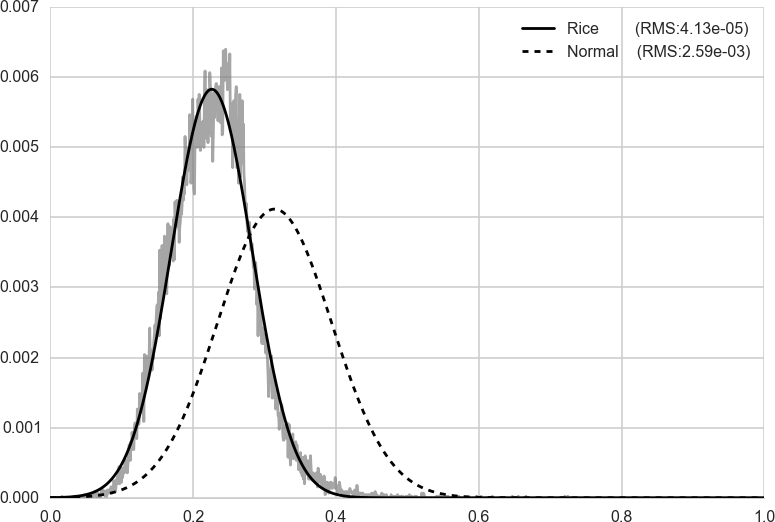
\includegraphics[width=0.48\textwidth]{5_normalization/figures/T2-normalization/03}}\hfill
  \subfigure[]{
    \label{fig:p2}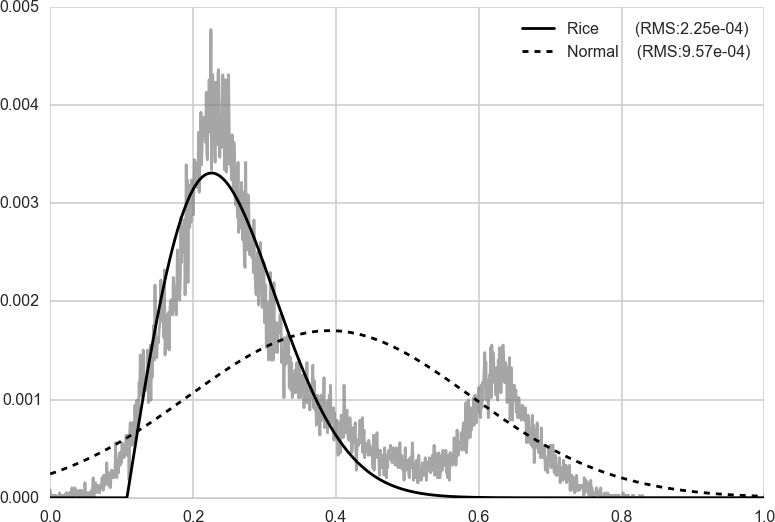
\includegraphics[width=0.48\textwidth]{5_normalization/figures/T2-normalization/06}}\hfill
%  \subfloat[][]{
%    \label{fig:p3}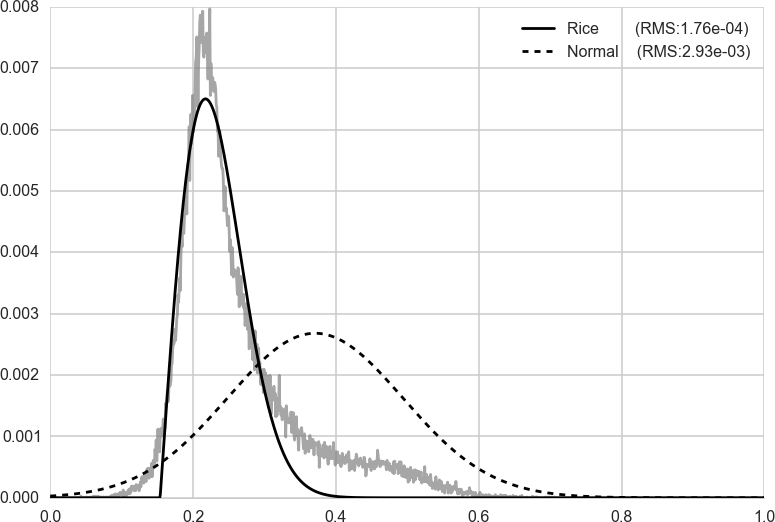
\includegraphics[width=0.3\textwidth]{14}}
  \caption{Visual evaluation of the goodness of fitting using Rician and Gaussian distribution.}
  \label{fig:fitting}
\end{figure}

The normalization is carried out as: 
(i) fit a Rician model to each prostate \ac{pdf} using non-linear least squares minimization; 
(ii) compute the mean (see~Eq.\,\eqref{eq:meanr}) and variance (see~Eq.\,\eqref{eq:var}) of the Rician model;
(iii) normalize the entire data using the \textit{z-score} similarly as in~Eq.\,\eqref{eq:zscore}.

\begin{equation}
  \mu_{r} = \sigma  \sqrt{\frac{\pi}{2}}\,\,L_{1/2}(-\frac{\nu^2}{2\sigma^2})  \ ,
  \label{eq:meanr}
\end{equation}

\begin{equation}
  \sigma_{r} = 2\sigma^2+\nu^2-\frac{\pi\sigma^2}{2}L_{1/2}^2\left(\frac{-\nu^2}{2\sigma^2}\right)  \ ,
  \label{eq:var}
\end{equation}

\noindent where $\nu$ and $\sigma$ are the distance between the reference point and the center of the bivariate distribution and the scale, respectively; $L_{1/2}$ denotes a Laguerre polynomial.

\subsubsection{Normalization using generative models in functional data analysis}\label{subsubsec:chp5:T2-norm:gen-model}

Srivastava \textit{et al.}~\cite{Srivastava2011} have proposed a generic method to register functional data, without any assumption regarding the models of different functions. 
This framework (see Sect.\,\ref{sec:regfra}) relies on the \ac{srsf} representation (see Sect.\,\ref{sec:srsf}) which transforms the Fisher-Rao metric into the conventional $\mathbb{L}^2$ metric, and thus allows to define a cost function corresponding to an Euclidean distance between two functions in this new representation.

\paragraph{\acl*{srsf} representation} \label{par:chp5:T2-norm:srsf}

In the proposed registration framework of functional data, two function $f_1$ and $f_2$ are registered by composing $f_2$ with a warping function $\gamma$ such that:

\begin{equation}
  \argmin_{\gamma \in \Gamma} D_{FR}(f_1, (f_2 \circ \gamma)) \ ,
  \label{eq:regfun}
\end{equation}

\noindent where $D_{FR}$ is the Fisher-Rao distance and $\Gamma$ is the set of all the functions $\gamma$.

The \Ac{srsf} representation is used to transform the functions and register them into this space.
The \ac{srsf} of a function $f$ is defined as:

\begin{equation}
  q(t) = \sign(\dot{f}(t))\sqrt{|\dot{f}(t)|} \ ,
  \label{eq:srsf}
\end{equation}

\noindent where $\dot{f}(t)$ corresponds to the derivative of $f$.

The major property of the \ac{srsf} representation used in the registration framework is the following: the composition of a function $f$ with a warping function $\gamma$ (i.e., $f \circ \gamma$) is equivalent to Eq.\,\eqref{eq:warp}, using the \ac{srsf} representation.

\begin{equation}
  \tilde{q}(t) = (q(t) \circ \gamma) \sqrt{\dot{\gamma}} \ ,
  \label{eq:warp}
\end{equation}

\noindent where $\dot{\gamma}$ is the derivative of $\gamma$.

Using this property, a cost function (named amplitude or $y$-distance) is defined to measure the similarity between two functions $f_1$ and $f_2$, expressed as in Eq.\,\eqref{eq:cf}

\begin{equation}
  D_y(f_1, f_2) = \underset{\gamma \in \Gamma}{\infspie} \| q_1 - (q_2 \circ \gamma) \sqrt{\dot{\gamma}} \| \ .
  \label{eq:cf}
\end{equation}

\paragraph{Registration framework}\label{par:chp5:T2-norm:regfra}

The registration framework consists into two steps. First, an initialization in which the Karcher mean $\mu_f$ is computed as in Eq.\,\eqref{eq:mean}

\begin{equation}
  \mu_f = \argmin_{f \in \mathcal{F}} \sum_{i = 1}^{n} D_y(f, f_i)^2 \ .
  \label{eq:mean}
\end{equation}

Then, for each function $f_i$: 
(i) compute $\gamma_{i}^{*}$ as in Eq.\,\eqref{eq:warpi}; 
(ii) compute $\tilde{q}_i$ as in Eq.\,\eqref{eq:warp};
(iii) update $\mu_f$ as in Eq.\,\eqref{eq:mean} by replacing $f_i$ by $\tilde{f_i}$, using $\tilde{q}_i$.

\begin{equation}
  \gamma_{i}^{*} = \argmin_{\gamma \in \Gamma} \sum_{i = 1}^{n} D_y(\mu_f, f_i)^2 \ ,
  \label{eq:warpi}
\end{equation}

\noindent where $n$ is the total number of functions to be aligned.

This step is iteratively performed based on the gradient of the cost function given in Eq.\,\eqref{eq:mean}. 
We refer the reader to the work of Srivastava\,\textit{et al.}~\cite{Srivastava2011} for more detailed discussion.


\subsection{Experiments and results}\label{subsec:chp5:T2-norm:Exp-res}

\subsubsection{Experiments}\label{subsub:chp5:T2-norm:res}
{\color{red}\textbf{This section has repetetive information according to data, it should be checked.}}

The experiments are conducted on a subset of public multi-parametric \ac{mri} prostate publicly available dataset\footnote{\url{http://visor.udg.edu/i2cvb/}}~\cite{lemaitre2015boosting}.
This dataset was acquired from a cohort of patients with higher-than-normal level of \ac{psa}. 
The acquisition was performed using a 3T whole body \ac{mri} scanner (Siemens Magnetom Trio TIM, Erlangen, Germany) using sequences to obtain \ac{t2w}-\ac{mri}. 
Aside of the \ac{mri} examinations, these patients also underwent a guided-biopsy. 
Finally, the dataset was composed of a total of 20 patients of which 18 patients had biopsy proven \ac{cap} and 2 patients were ``healthy'' with negative biopsies. 
In this study, our subset consists of 17 patients with \ac{cap}. 
The prostate organ as well as the prostate zones (i.e., \ac{pz}, \ac{cg}) and \ac{cap} were manually segmented by an experienced radiologist.

The different normalization methods are implemented in Python and publicly available in GitHub\footnote{\url{https://github.com/glemaitre/protoclass}}.
The normalization based on \ac{srsf} uses the implementation\footnote{\url{https://bitbucket.org/tetonedge/fdasrsf}} of Tucker\,\textit{et al.}~\cite{Tucker2013}.

The model fitting for the Gaussian and Rician normalization is performed as a non-linear least squares problem, using Levenberg-Marquardt optimization.
The piecewise-linear normalization is performed using the following set of percentiles $s \in \{0, 5, 25, 50, 75, 95, 100 \}$ as landmarks.
In the \ac{srsf}-based normalization, the \acp{pdf} are smoothed using spline-based denoising method.

\subsubsection{Results}\label{subsub:chp5:T2-norm:res}
\paragraph{Qualitative}

\begin{figure}
  \centering
  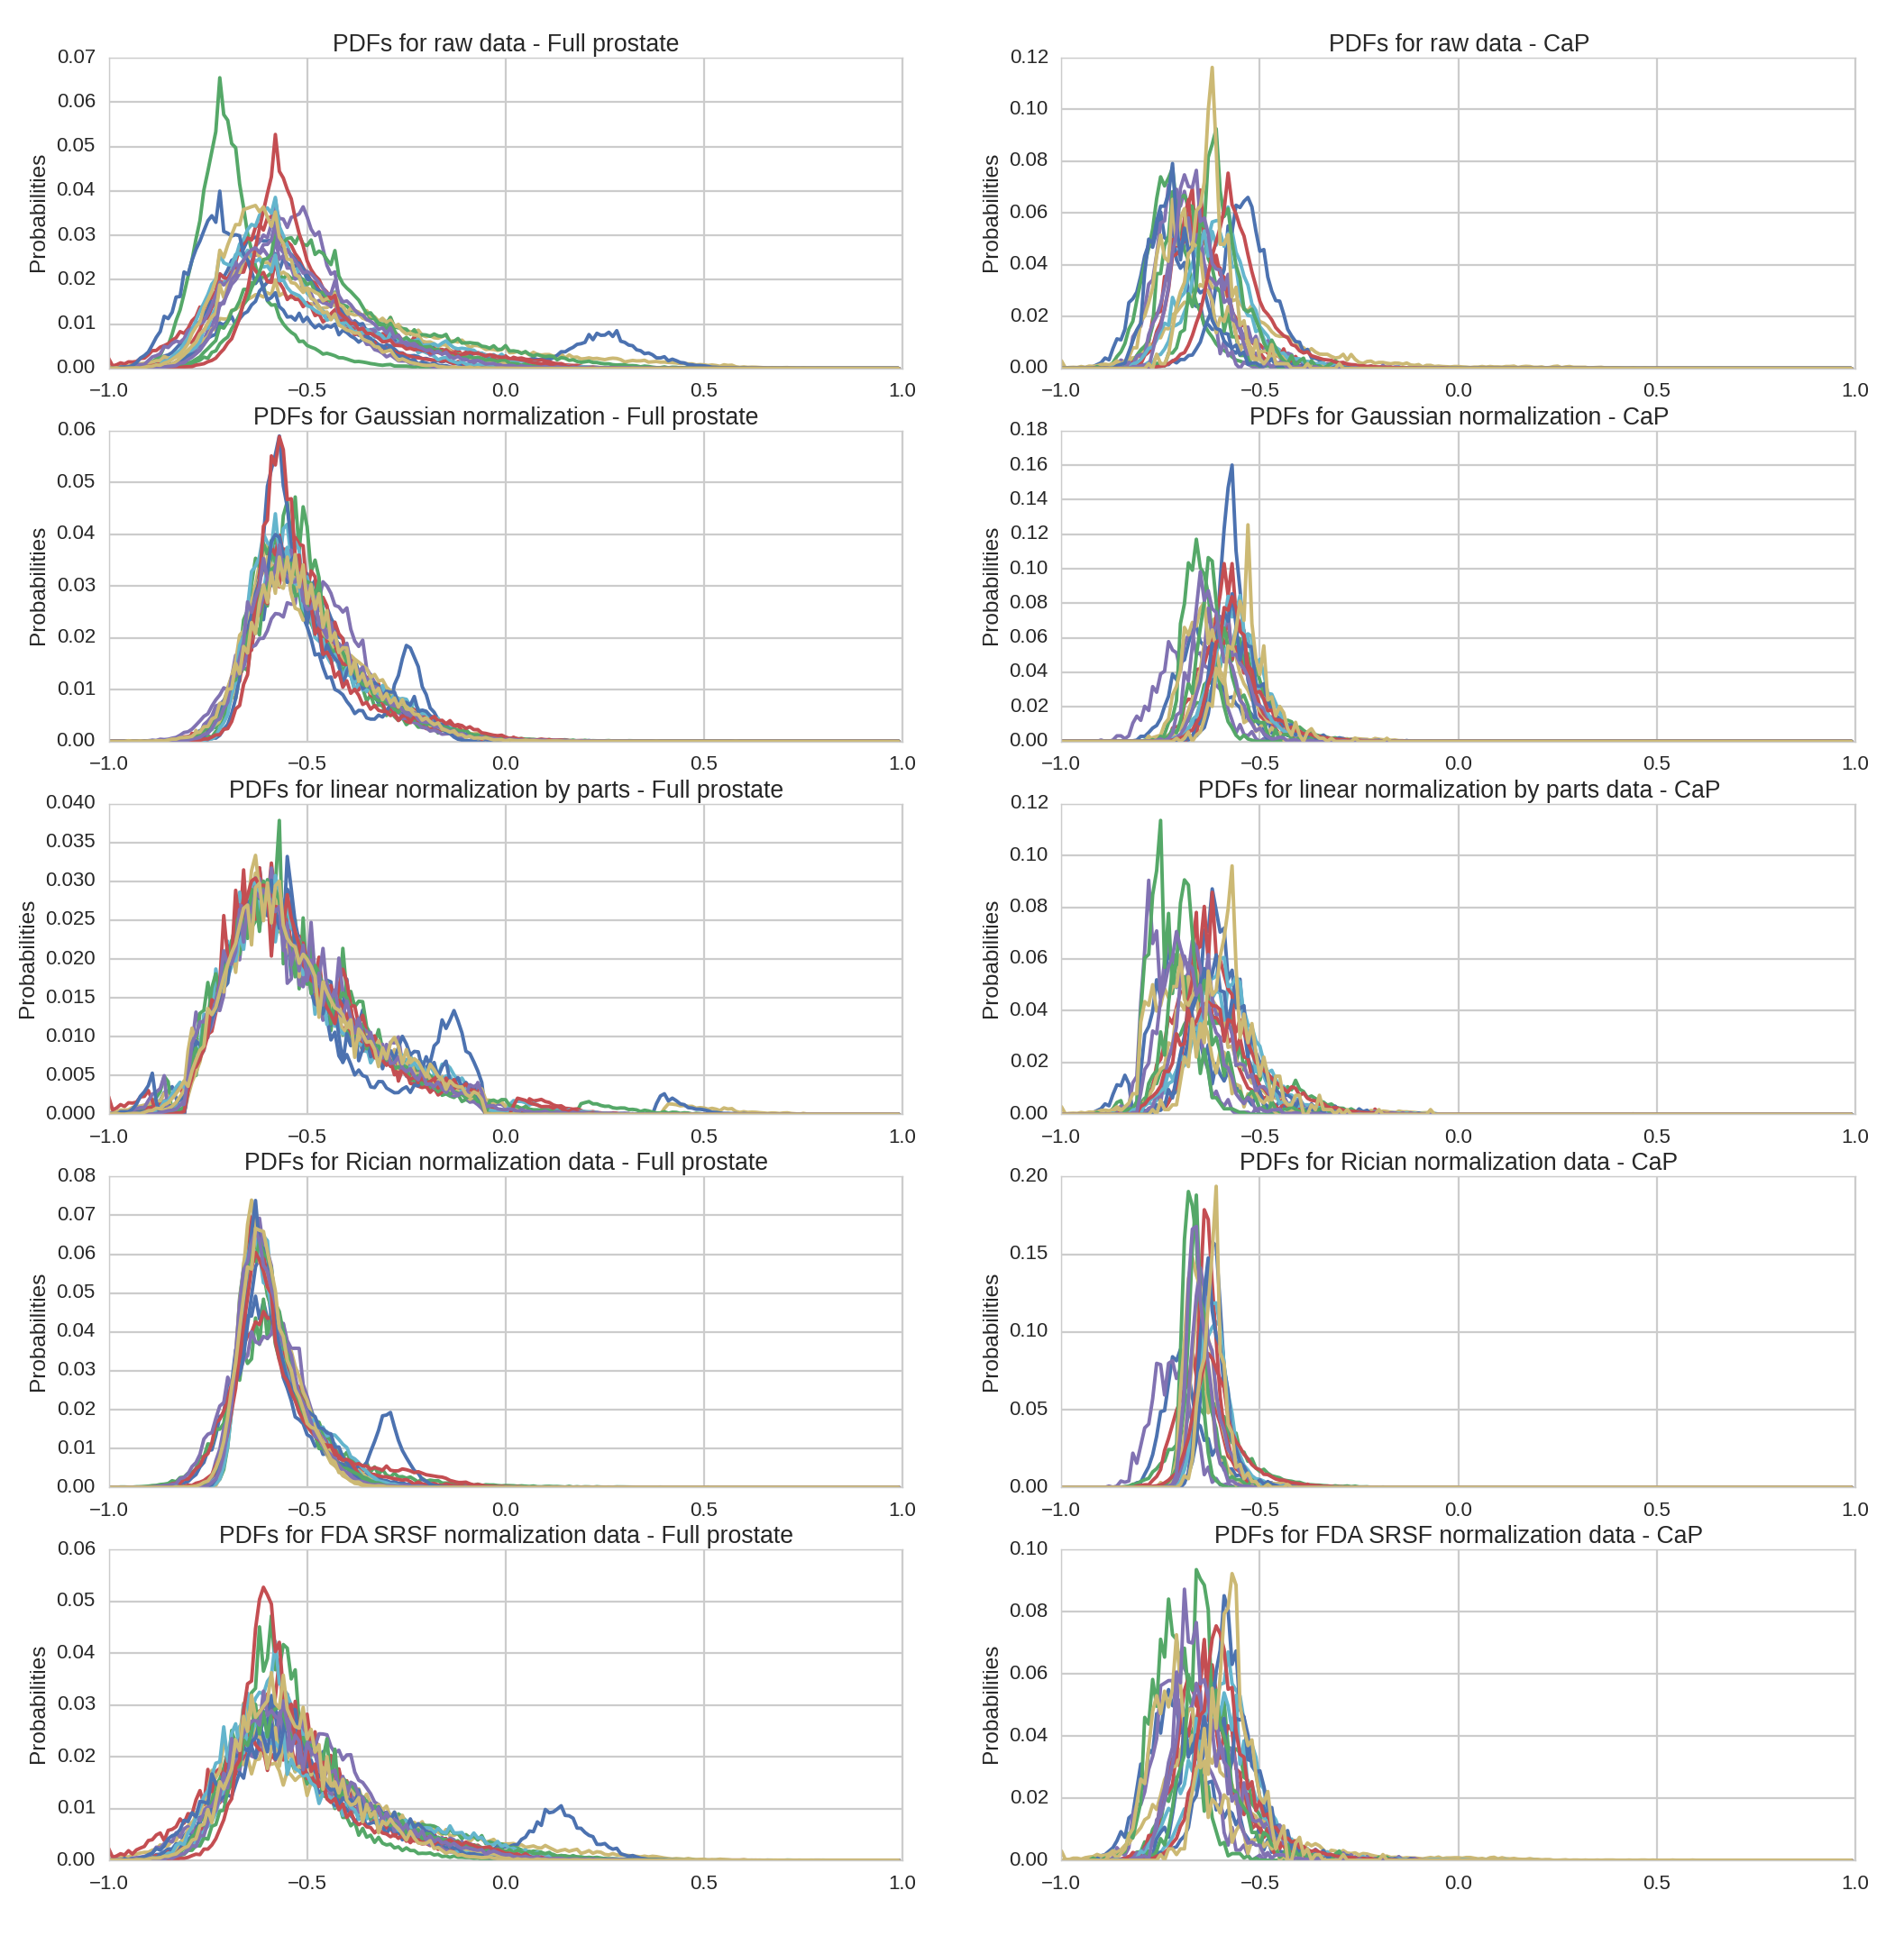
\includegraphics[width=1.\textwidth]{5_normalization/figures/T2-normalization/qualitative.png}
  \caption{Qualitative evaluation by visual inspection of the alignment of the \ac{pdf}s for the full prostate and the \ac{cap}.}
  \label{fig:qu}
\end{figure}

Figure~\ref{fig:qu} depicts the alignment of the different \ac{pdf}s using the different methods implemented. 
All the methods seem to address the problem of the \ac{pdf} alignment of the full prostate data.
However, the Rician normalization seems to outperform the other methods when focusing solely on the \ac{cap} data.
The \ac{pdf} computed in this specific area is more skewed from its original shape in the case of the piecewise-linear normalization than with the three other normalization strategies.
The \ac{srsf} normalization gets unstable due to the warping function $\gamma$ found which is in practise non-smooth.

\paragraph{Quantitative}

\begin{figure}
  \centering
  \subfigure[]{
    \label{fig:qtfull}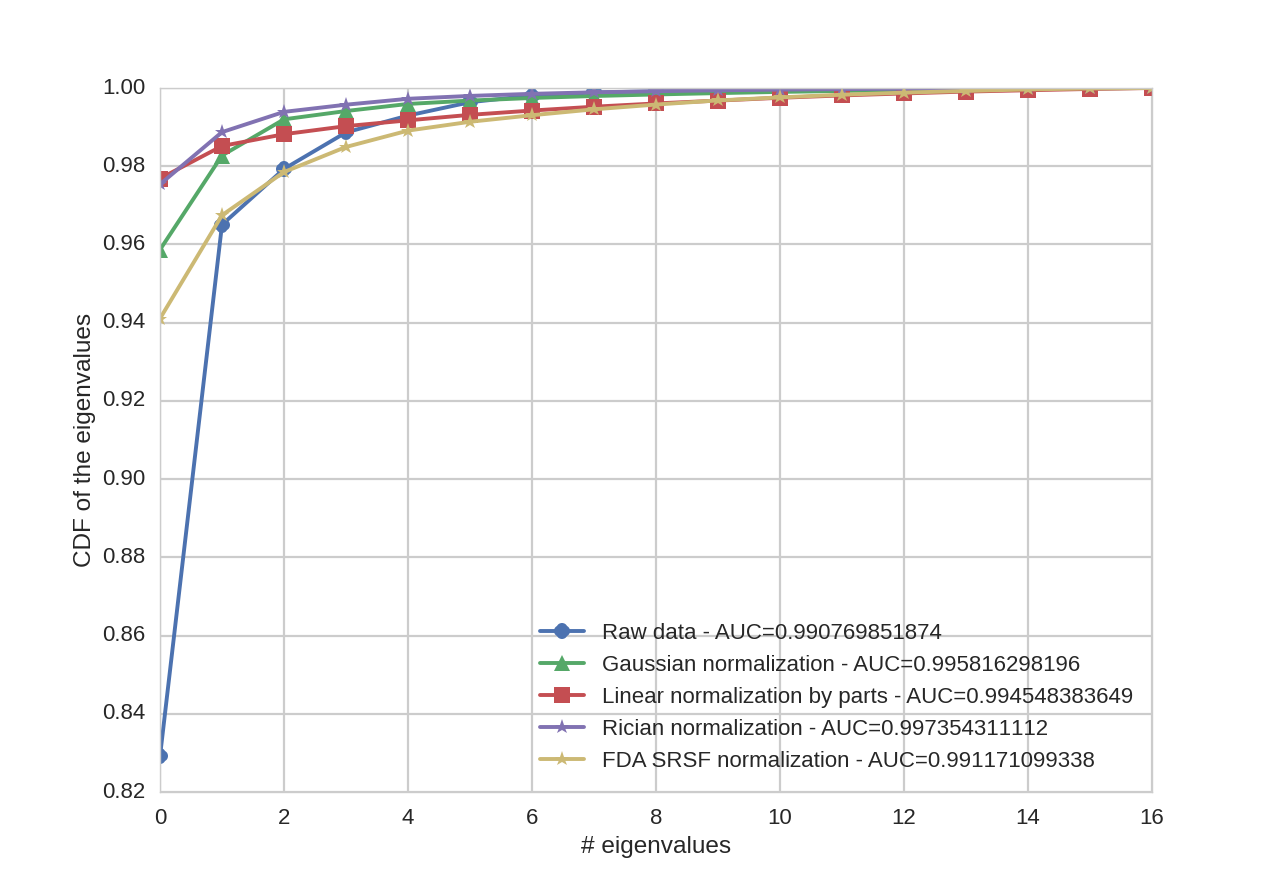
\includegraphics[width=0.8\textwidth]{5_normalization/figures/T2-normalization/quantitative_1.png}}\hfill
  \subfigure[]{
    \label{fig:qtcap}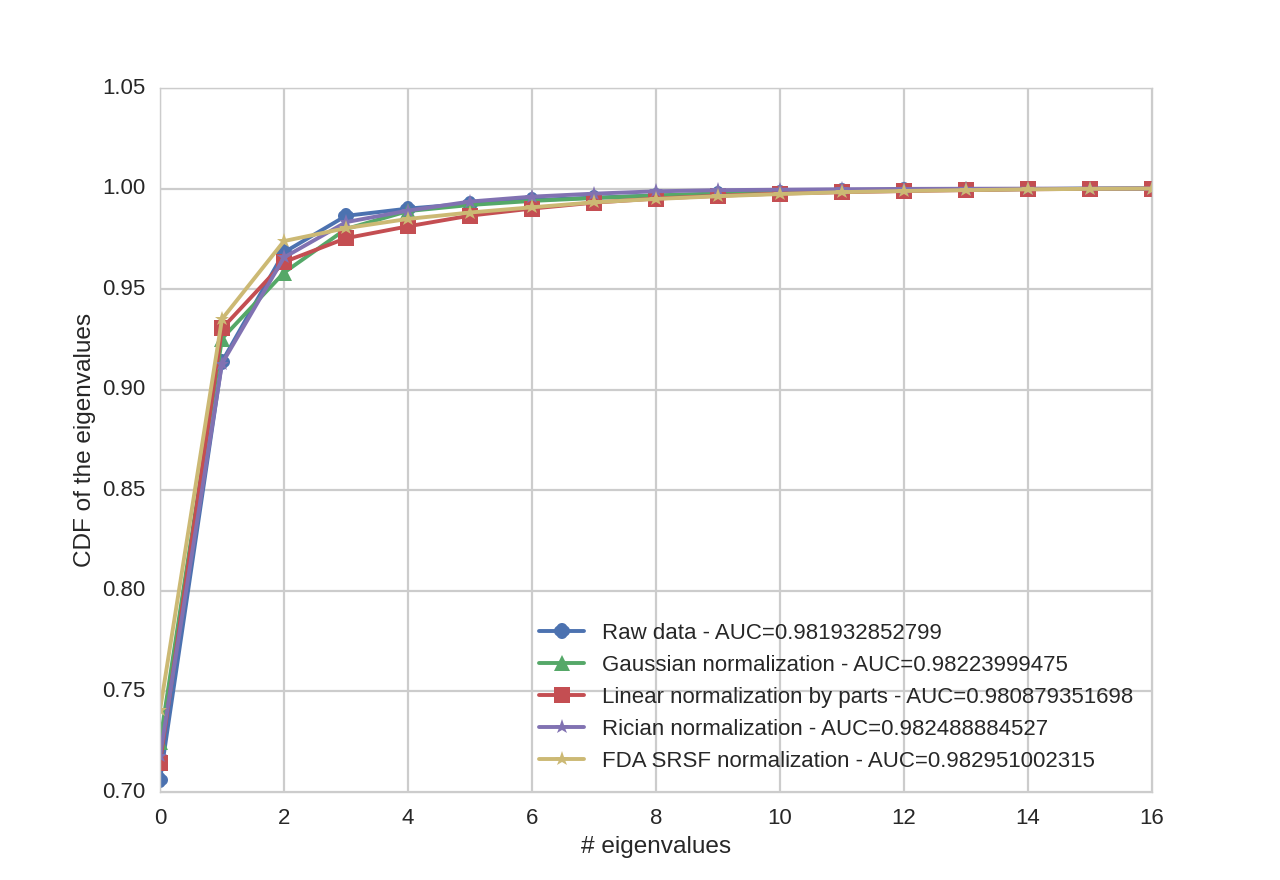
\includegraphics[width=0.8\textwidth]{5_normalization/figures/T2-normalization/quantitative_2.png}}
  \caption{Spectral evaluation using \ac{pca} decomposition: \protect\subref{fig:qtfull} evaluation considering the full prostate, \protect\subref{fig:qtcap} evaluation considering only the \ac{cap}.}
  \label{fig:qt}
\end{figure}

A spectral evaluation is performed by decomposing the set of normalized \ac{pdf}s using \ac{pca} under the assumption that they are linearly dependent. 
Intuitively, the eigenvalues of the \ac{pca} decomposition are correlated with the alignment of the different \ac{pdf}s.
Thus, in the case of a perfect alignment of the \ac{pdf}s, the first eigenvalue is much greater than the remaining since that the first eigenvector encodes all the information.
In the contrary, in the case of a misalignment of the \ac{pdf}s, more eigenvectors are needed to encode the information synonymous with larger eigenvalues.
Thus, we propose to use the cumulative sum of the normalized eigenvalues as well as the \ac{auc}, as depicted in Fig.\,\ref{fig:qt}.
Rician normalization outperforms the other methods with an \ac{auc} of $0.9974$ and $0.9824$ considering the full prostate and \ac{cap}, respectively.

\subsection{Discussion and conclusion}\label{subsec:chp5:T2-norm:dis-con}
In this section, we propose to normalize the \ac{t2w}-\ac{mri} prostate images using two new strategies: (i) based on a Rician \textit{a priori} and (ii) based on a \ac{srsf} representation which do not make any assumption regarding the \ac{pdf} of the data.
An extensive comparison was conducted showing that the Rician normalization outperforms the Gaussian, \ac{srsf}-based, and piecewise-linear normalization for \ac{t2w}-\ac{mri} prostate images normalization.

As avenues for future research, the contribution of the Rician normalization must be evaluated in a classification framework. Furthermore, normalized \ac{t2w}-\ac{mri} can be included with other modalities in order to perform classification using multi-parametric \ac{mri} data.

